\documentclass[reprint,amsmath,amssymb,aps,prb]{revtex4-2}
\usepackage{graphicx}
\begin{document}
\onecolumngrid

\vspace*{1cm}
\begin{center}
  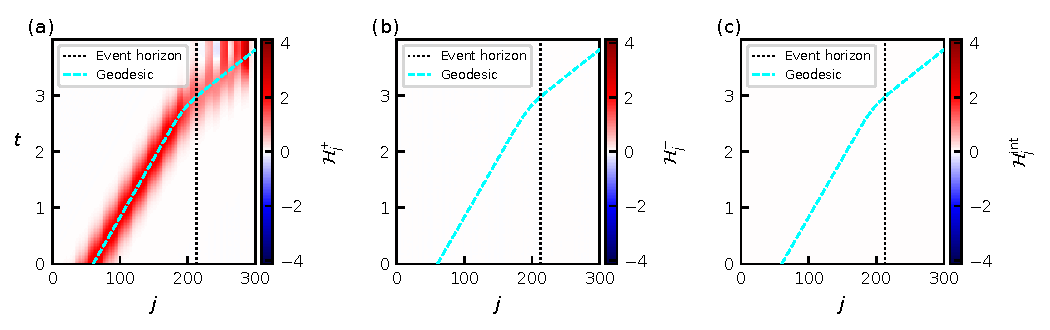
\includegraphics[width=\textwidth]{composites/fig02_p0_aplus.pdf}\par
  \small Proposed Fig.~2 at full two-column width.
\end{center}
\newpage

\vspace*{1cm}
\begin{center}
  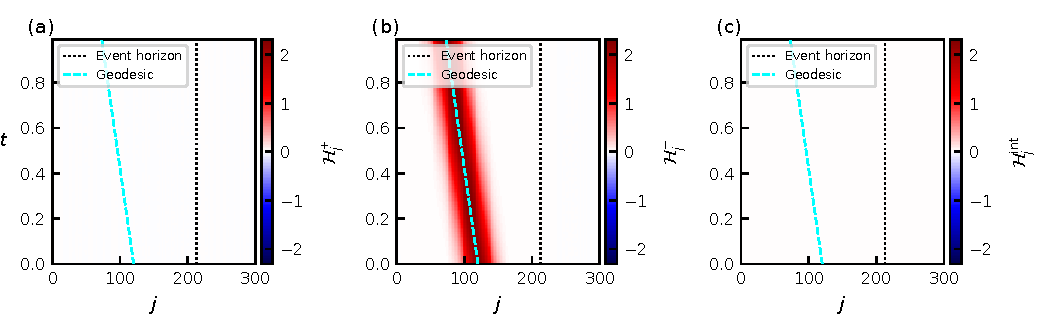
\includegraphics[width=\textwidth]{composites/fig03_p0_aminus.pdf}\par
  \small Proposed Fig.~3 at full two-column width.
\end{center}
\newpage

\vspace*{1cm}
\begin{center}
  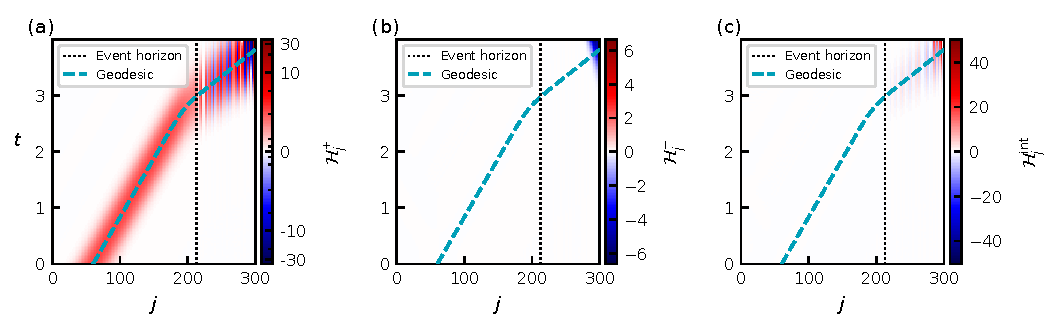
\includegraphics[width=\textwidth]{composites/fig04_p1_aplus.pdf}\par
  \small Proposed Fig.~4 at full two-column width.
\end{center}
\newpage

\vspace*{1cm}
\begin{center}
  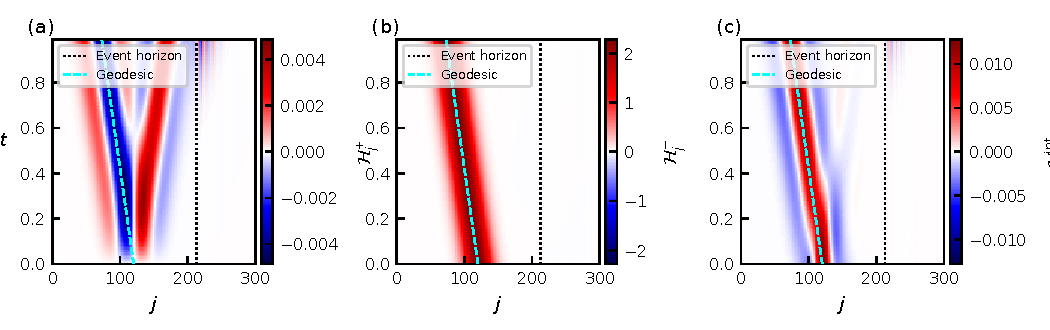
\includegraphics[width=\textwidth]{composites/fig05_p1_aminus.pdf}\par
  \small Proposed Fig.~5 at full two-column width.
\end{center}
\newpage

\vspace*{1cm}
\noindent\begin{minipage}{0.48\textwidth}
  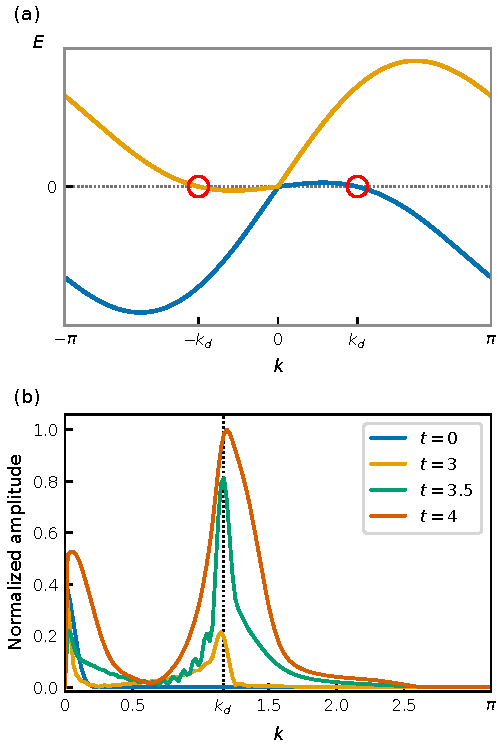
\includegraphics[width=\linewidth]{single_column_candidates/doubler_fft_vertical.pdf}\par
  \small Single-column vertical candidate: doubler and FFT.
\end{minipage}
\newpage

\vspace*{1cm}
\noindent\begin{minipage}{0.48\textwidth}
  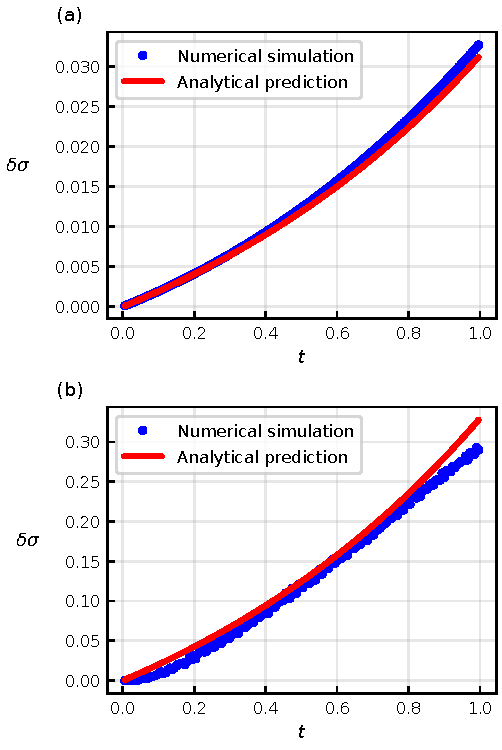
\includegraphics[width=\linewidth]{single_column_candidates/surface_gravity_vertical.pdf}\par
  \small Single-column vertical candidate: surface gravity.
\end{minipage}
\newpage

\vspace*{1cm}
\noindent\begin{minipage}{0.48\textwidth}
  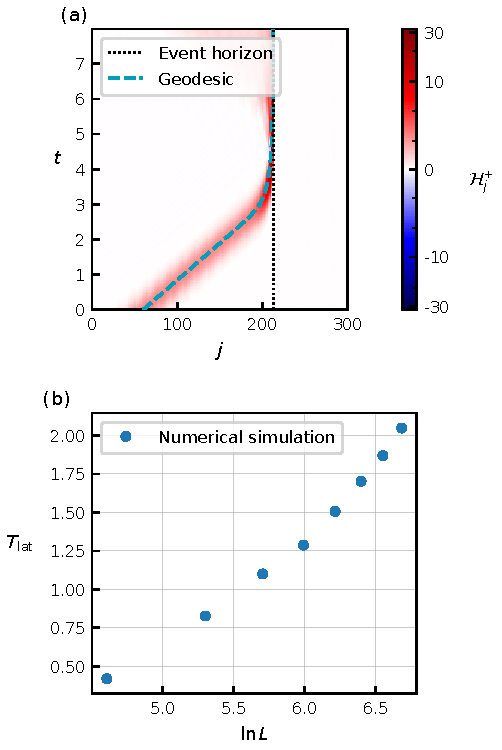
\includegraphics[width=\linewidth]{single_column_candidates/WH_p0_vertical.pdf}\par
  \small Single-column vertical candidate: white hole at $p=0$.
\end{minipage}
\newpage

\vspace*{1cm}
\noindent\begin{minipage}{0.48\textwidth}
  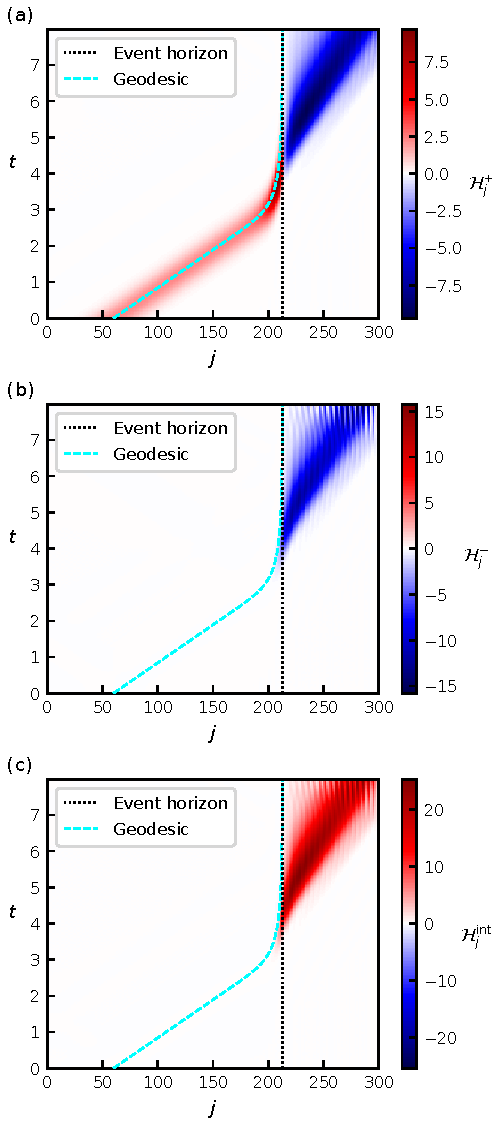
\includegraphics[width=\linewidth]{single_column_candidates/WH_p1_vertical.pdf}\par
  \small Single-column vertical candidate: white hole at $p=1$.
\end{minipage}

\end{document}
